\section{Generative Models}

Generative models aim to model the joint probability distribution \( P(x, y) \) over inputs \( x \) and labels \( y \).  
By Bayes' theorem:
\[
P(x, y) = P(x \mid y) P(y)
\]
They attempt to learn the underlying structure of the data — allowing inference of missing labels, anomaly detection, and generation of new (synthetic) samples.

Given training data:
\[
T = \{ (x_i, y_i) \}_{i=1}^{n}
\]
we aim to generalize from the observed data to find a hypothesis \( h(x) \in \mathcal{H} \) that minimizes a suitable loss function.

---

\subsection{Gaussian Mixture Models (GMMs)}

A \textbf{Gaussian Mixture Model (GMM)} assumes that the data are generated from a mixture of \( K \) Gaussian distributions:
\[
P(x) = \sum_{k=1}^{K} \pi_k \, \mathcal{N}(x \mid \mu_k, \Sigma_k)
\]
where:
\begin{itemize}
    \item \( \pi_k \) is the mixture coefficient (\( \sum_k \pi_k = 1 \)),
    \item \( \mu_k \) is the mean of cluster \( k \),
    \item \( \Sigma_k \) is the covariance of cluster \( k \),
    \item \( \mathcal{N}(x \mid \mu_k, \Sigma_k) \) is the multivariate Gaussian PDF.
\end{itemize}

Each class or cluster is represented as a multivariate Gaussian distribution.  
The model can describe both separate and overlapping clusters, as shown below.

\begin{figure}[h]
\centering
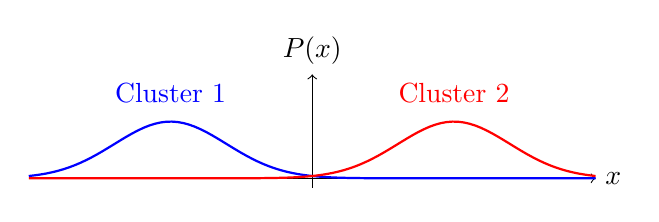
\begin{tikzpicture}[scale=1.2]
% Axes
\draw[->] (-3,0) -- (3,0) node[right] {$x$};
\draw[->] (0,-0.1) -- (0,1.1) node[above] {$P(x)$};

% Two Gaussian curves
\draw[thick,blue,domain=-3:3,samples=100] 
  plot (\x,{0.6*exp(-(\x+1.5)^2/0.7)});
\draw[thick,red,domain=-3:3,samples=100] 
  plot (\x,{0.6*exp(-(\x-1.5)^2/0.7)});

% Labels
\node[blue] at (-1.5,0.9) {Cluster 1};
\node[red] at (1.5,0.9) {Cluster 2};
\end{tikzpicture}
\caption{Two clusters represented by Gaussian components in a GMM. Overlap between clusters indicates probabilistic (soft) boundaries.}
\end{figure}

---

\subsection{Supervised, Unsupervised, and Semi-supervised Learning}

GMMs and K-Means can both be used for clustering:

\begin{itemize}
    \item \textbf{K-Means:} hard assignments — each point belongs to one cluster.
    \item \textbf{GMM:} soft assignments — each point has a probability of belonging to each cluster.
\end{itemize}

\textbf{GMMs can be used for:}
\begin{itemize}
    \item \textbf{Unsupervised learning:} to discover latent clusters in unlabeled data.
    \item \textbf{Supervised learning:} to estimate class-conditional distributions \( P(x \mid y) \).
    \item \textbf{Semi-supervised learning:} to combine labeled and unlabeled data.
\end{itemize}

\textbf{Semi-supervised GMM Algorithm:}
\begin{enumerate}
    \item Learn the initial GMM from available (labeled + unlabeled) data.
    \item Predict missing labels using the current model (e.g., via QDA or posterior probability).
    \item Update the GMM using all data (including predicted labels).
    \item Repeat until convergence (the loss no longer decreases).
\end{enumerate}

\begin{figure}[h]
\centering
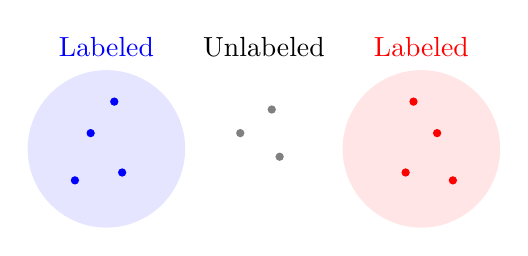
\begin{tikzpicture}[scale=1.0]
% Two clusters
\fill[blue!20,opacity=0.5] (-2,0) circle (1);
\fill[red!20,opacity=0.5] (2,0) circle (1);
% Points
\foreach \x/\y in {-2.2/0.2, -1.8/-0.3, -2.4/-0.4, -1.9/0.6} {
  \fill[blue] (\x,\y) circle (1.5pt);
}
\foreach \x/\y in {2.2/0.2, 1.8/-0.3, 1.9/0.6, 2.4/-0.4} {
  \fill[red] (\x,\y) circle (1.5pt);
}
% Unlabeled
\foreach \x/\y in {-0.3/0.2, 0.2/-0.1, 0.1/0.5} {
  \fill[gray] (\x,\y) circle (1.5pt);
}
\node at (-2,1.3) {\textcolor{blue}{Labeled}};
\node at (2,1.3) {\textcolor{red}{Labeled}};
\node at (0,1.3) {Unlabeled};
\end{tikzpicture}
\caption{Semi-supervised data distribution: labeled and unlabeled points.}
\end{figure}

---

\subsection{Choosing the Number of Clusters (Elbow Method)}

The \textbf{elbow method} is used to select the optimal number of clusters \( K \). It plots the within-cluster sum of squares (WCSS) versus \( K \).  
The ``elbow'' point indicates where adding more clusters provides diminishing returns.

\begin{figure}[h]
\centering
\begin{tikzpicture}[scale=1.0]
% Axes
\draw[->] (0,0) -- (5,0) node[right] {$K$};
\draw[->] (0,0) -- (0,3.2) node[above] {WCSS};
% Curve
\draw[thick,blue,domain=1:4.5,smooth] plot (\x,{3/(0.8*\x+0.5)+0.2});
% Dots
\foreach \x in {1,2,3,4} {
  \fill[blue] (\x,{3/(0.8*\x+0.5)+0.2}) circle (1.5pt);
}
\node[above right,blue] at (2,1.9) {Elbow point};
\draw[dashed] (2,0) -- (2,2);
\end{tikzpicture}
\caption{Elbow method: the optimal $K$ occurs at the elbow point where reduction in error slows down.}
\end{figure}

---

\subsection{Anomaly Detection with GMMs}

GMMs can detect anomalies by identifying points with very low probability density.

Let \( P(x_{\text{test}}) \) be the probability density of a test observation.  
If
\[
P(x_{\text{test}}) < \epsilon
\]
for some threshold \( \epsilon \), the observation is classified as an \textbf{anomaly}.

\textbf{Applications:}
\begin{itemize}
    \item Fraud detection (e.g., credit card transactions)
    \item Aircraft health monitoring (heat, vibration)
    \item Data center metrics:
    \begin{itemize}
        \item \( x_1 \): memory usage
        \item \( x_2 \): disk space
        \item \( x_3 \): CPU load
        \item \( x_4 \): network traffic
    \end{itemize}
\end{itemize}

\begin{figure}[h]
\centering
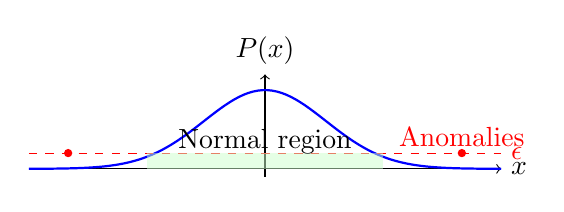
\begin{tikzpicture}[scale=1.0]
% Axes
\draw[->] (-3,0) -- (3,0) node[right] {$x$};
\draw[->] (0,-0.1) -- (0,1.2) node[above] {$P(x)$};

% Gaussian
\draw[thick,blue,domain=-3:3,samples=100] plot (\x,{exp(-(\x)^2/1.2)});
% Threshold
\draw[dashed,red] (-3,0.2) -- (3,0.2) node[right] {$\epsilon$};
% Normal region
\fill[green!20,opacity=0.5] (-1.5,0) rectangle (1.5,0.2);
\node at (0,0.35) {Normal region};
% Anomalies
\fill[red] (-2.5,0.2) circle (1.5pt);
\fill[red] (2.5,0.2) circle (1.5pt);
\node[red] at (2.5,0.4) {Anomalies};
\end{tikzpicture}
\caption{Anomaly detection using GMM: data points below the probability threshold $\epsilon$ are marked as anomalies.}
\end{figure}

---

\subsection{Synthetic Data Generation}

Generative models can also create new synthetic data points from the learned distribution \( P(x) \).  
This can enhance model performance when labeled data are scarce, helping improve cluster separation and classification accuracy.

---

\subsection{Summary and Exam Notes}

\begin{itemize}
    \item Generative models learn \( P(x, y) = P(x \mid y) P(y) \).
    \item GMMs assume data are generated from a mixture of Gaussians.
    \item GMMs can be used for supervised, unsupervised, and semi-supervised learning.
    \item Use the elbow method to determine the number of clusters.
    \item Anomalies are detected when \( P(x_{\text{test}}) < \epsilon \).
    \item Example question: \textit{``What method can handle semi-supervised data?''} → \textbf{GMM (Gaussian Mixture Model)}.
\end{itemize}
